% This is a LaTeX template (version from 2016 Feb. 17) 
% for preparing documents for All-Russian Scientific Conference 
% of the Mathematical Modeling and Boundary Value Problems 
% [Matem. Mod. Kraev. Zadachi, Samara, Russian Federation]. 
%
% It was submitted by an author writing for 
% the 10th All-Russian Scientific Conference with 
% international participation (MMiKZ’16).
%
% The various components of your paper [title, text, heads, etc.] 
% are already defined on the style sheet, as illustrated 
% by the portions given in this document.
%
% Author: Mikhail N. Saushkin (msaushkin@gmail.com)
% License: Creative Commons CC BY 4.0 
% <https://creativecommons.org/licenses/by/4.0/>

\documentclass[10pt,twoside,book,a5paper]{ncc}
\usepackage[utf8]{inputenc}
\usepackage[english,russian]{babel}
\usepackage{indentfirst}

% This is a macro definition (version from 2016 Feb. 17) for a LaTeX template 
% for preparing documents for All-Russian Scientific Conference 
% of the Mathematical Modeling and Boundary Value Problems 
% [Matem. Mod. Kraev. Zadachi, Samara, Russian Federation]. 
%
% It was submitted by an author writing for 
% the 10th All-Russian Scientific Conference with 
% international participation (MMiKZ’16).
%
% Author: Mikhail N. Saushkin (msaushkin@gmail.com)
% License:  LaTeX Project Public License (LPPL) 
% <http://latex-project.org/lppl/>

% Dear authors of the MMiKZ’16 Conference, please do not make changes into this file.

\usepackage[a5paper, mag=1000, left=1.5cm, right=1.5cm, top=1cm, bottom=2cm, headsep=0.7cm, footskip=1cm]{geometry}
\usepackage{ifthen}
\usepackage{xcolor}
\usepackage{amsbib}
\usepackage{amsmath}
\usepackage{amssymb}
%\usepackage[colorlinks]{hyperref} 
% this package can by loaded in the amsbib package
\usepackage{nccfancyhdr}
\usepackage{mathtools}
\mathtoolsset{showonlyrefs}
\usepackage{epstopdf}
\usepackage[sort,compress]{cite}
%\usepackage{textcase} 
% this does not work with an utfx inputenc codepage for cyrillic letters

\makeatletter\@logosfalse\makeatother % we don't show amsbib package logos

\pagestyle{fancy}
\fancyhead{}
\fancyhead[RO,LE]{}
\fancyfoot{}
\fancyfoot[LE,RO]{\thepage}
\fancyfoot[LO,CE]{}
\fancyfoot[CO,RE]{}
\renewcommand{\headrulewidth}{0pt}
\renewcommand{\footrulewidth}{0pt}

\newcommand{\udc}{}
\newcommand{\theudc}{}
\renewcommand{\udc}[1]{%
\renewcommand{\theudc}{{\noindent\small \CYRU\CYRD\CYRK~#1}}}

\newcommand{\thetitle}{}
\newcommand{\TitleInTitlePage}{}
\newcommand{\TitleInTableOfContenst}{}
\renewcommand{\title}[1]{%
\renewcommand{\thetitle}{#1}%
%\renewcommand{\TitleInTitlePage}{{\small\bf\MakeTextUppercase{#1}}} 
% this does not work with an utfx inputenc codepage for cyrillic letters
\renewcommand{\TitleInTitlePage}{{\large\sc{#1}}}%
\renewcommand{\TitleInTableOfContenst}{\noindent {#1}}}

\newcommand{\theauthor}{}
\newcommand{\AutorInTitlePage}{}
\newcommand{\AuthorInTableOfContenst}{}
\renewcommand{\author}[2]{%
\renewcommand{\theauthor}{{\footnotesize\sl #1}}%
\renewcommand{\AutorInTitlePage}{{\noindent{\emph{#1}}}}%
\renewcommand{\AuthorInTableOfContenst}{#2}}

\newcommand{\ac}[2]{\addcontentsline{toc}{chapter}{{\it #1} #2}}

\newcounter{figure} % is it a ncc class trouble?
\newcounter{table}  % is it a ncc class trouble?
\newcounter{thm}
\newcounter{rem}
\newcounter{exa}
\newcounter{lem}
\newcounter{def}

\newcommand{\clean}{
\setcounter{section}{0}
\setcounter{thm}{0}
\setcounter{rem}{0}
\setcounter{exa}{0}
\setcounter{lem}{0}
\setcounter{def}{0}
\setcounter{equation}{0}
\setcounter{figure}{0}
\setcounter{table}{0}
\setcounter{footnote}{0}
}

\providecommand\phantomsection{} 

\renewcommand{\maketitle}{%
\vspace{1cm plus 1ex minus .2ex}
\phantomsection
\ac{\AuthorInTableOfContenst~\nobreak}{\TitleInTableOfContenst} 
\clean
\theudc
\begin{center}
\AutorInTitlePage 
\vskip1mm 
\TitleInTitlePage
\end{center} 
\normalsize 
\normalfont
\vskip1mm}

\newcommand{\email}[1]{\href{mailto:#1}{\texttt{\nolinkurl{#1}}}}

\DeclareSection*{1}{section}{}{0.5ex plus 1ex minus .2ex}{0.3ex plus.2ex}{\normalsize\bff}
\DeclareSection{-1}{figure}{\rm}{2.5ex}{0pt}{\small}
\DeclareSection{-2}{table}{\small\sc}{0pt}{0.5ex}{\small}
\renewcommand{\thempfootnote}{\it\alph{mpfootnote}} % 
% a \ralph command is default in the russian definition for \thempfootnote command, 
% so we have a trouble with this in the mathematical mode
\renewcommand{\theequation}{\arabic{equation}}
\renewcommand{\thesection}{\arabic{section}}
\renewcommand{\thefigure}{\rm \arabic{figure}}
\DeclareTOCEntry{0}{}{}{9.9}{}
\setcounter{tocdepth}{0}
\SectionTagSuffix{.~}
\sectionstyle{center}
\captiontagstyle[table]{right}
\captionstyle{centerlast}

\newcommand{\Proof}{\vskip1mm\textit{\CYRD\cyro\cyrk\cyra\cyrz\cyra\cyrt\cyre\cyrl\cyrsftsn\cyrs\cyrt\cyrv\cyro\/~}}
\renewenvironment{proof}[1][s]
{\vskip1mm \ifthenelse{\equal{#1}{s}}{{\it \CYRD\cyro\cyrk\cyra\cyrz\cyra\cyrt\cyre\cyrl\cyrsftsn\cyrs\cyrt\cyrv\cyro\/}.~}{{#1. }}}{\hfill$\scriptstyle\square$
\vskip1mm}

\newenvironment{newthm}[2][s]
{\vskip1mm \ifthenelse{\equal{#1}{s}}{{\small \sc #2.}}{{\small \sc #2 #1.}}}{\vskip1mm}

\renewenvironment{theorem}[1][s]
{\vskip1mm\ifthenelse{\equal{#1}{s}}{\refstepcounter{thm}{\small\sc\CYRT\cyre\cyro\cyrr\cyre\cyrm\cyra~\thethm.~}\it}
{{\small\sc\CYRT\cyre\cyro\cyrr\cyre\cyrm\cyra~#1.}\it}}{\vskip1mm}
\newenvironment{theorem*}
{\vskip1mm{\small\sc\CYRT\cyre\cyro\cyrr\cyre\cyrm\cyra.}\it}{\vskip1mm}

\renewenvironment{remark}[1][s]
{\vskip1mm \ifthenelse{\equal{#1}{s}}{\refstepcounter{rem}{\small\sc\CYRZ\cyra\cyrm\cyre\cyrch\cyra\cyrn\cyri\cyre~\therem.~}}
{{\small\sc\CYRZ\cyra\cyrm\cyre\cyrch\cyra\cyrn\cyri\cyre~#1.~}}}{\vskip1mm}
\newenvironment{remark*}
{\vskip1mm{\small\sc\CYRZ\cyra\cyrm\cyre\cyrch\cyra\cyrn\cyri\cyre.~}}{\vskip1mm}

\renewenvironment{example}[1][s]
{\vskip1mm \ifthenelse{\equal{#1}{s}}{\refstepcounter{exa}{\small\sc\CYRP\cyrr\cyri\cyrm\cyre\cyrr~\theexa.}}
{{\small\sc\CYRP\cyrr\cyri\cyrm\cyre\cyrr~#1.}}}{\vskip1mm}
\newenvironment{example*}
{\vskip1mm{\small\sc\CYRP\cyrr\cyri\cyrm\cyre\cyrr.}}
{\vskip1mm}

\renewenvironment{lemma}[1][s]
{\vskip1mm \ifthenelse{\equal{#1}{s}}{\refstepcounter{lem}{\small\sc \CYRL\cyre\cyrm\cyrm\cyra~\thelem.~}}
{{\small\sc \CYRL\cyre\cyrm\cyrm\cyra~#1.}}}{\vskip1mm}
\newenvironment{lemma*}
{\vskip1mm {\small\sc \CYRL\cyre\cyrm\cyrm\cyra.}}{\vskip1mm}

\renewenvironment{definition}[1][s]
{\vskip1mm \ifthenelse{\equal{#1}{s}}{\refstepcounter{def}{\small\sc\CYRO\cyrp\cyrr\cyre\cyrd\cyre\cyrl\cyre\cyrn\cyri\cyre~\thedef.~}}
{{\small\sc\CYRO\cyrp\cyrr\cyre\cyrd\cyre\cyrl\cyre\cyrn\cyri\cyre~#1.}}}{\vskip1mm}
\newenvironment{definition*}
{\vskip1mm{\small\sc\CYRO\cyrp\cyrr\cyre\cyrd\cyre\cyrl\cyre\cyrn\cyri\cyre.~}}{\vskip1mm}
% Убедительная просьба к авторам не редактировать файл definition.tex 
% и не вводить свои макроопределения. 
% Вы можете подключить дополнительные пакеты, 
% не изменяющие работу уже подключенных.

\begin{document}

% Вы можете удалить любые комментарии, если они мешают Вам при наборе рукописи. 
\udc{51:061.2/.3:004.4\protect\footnote{Рукопись должна содержать УДК, который рекомендуется брать из следующего источника:
\url{http://www.mathnet.ru/udc.pdf}.}} 
%\udc{51:061.2/.3:004.4}
% Укажите индекс УДК, соответствующий Вашей работе.

\title{Шаблон оформления рукописи доклада на~конференцию~ММиКЗ'16\protect\footnote{\color{red}Внимание! Авторы сами в праве выбирать название секций и их содержимое, в~шаблоне секционирование приводится как образец!}}
%\title{Название Вашей статьи}
%% Название работы пишется строчными буквами начиная с Прописной буквы.

\author{М.~Н.~Саушкин}{Саушкин~М.~Н.}
% Автор(ы) через запятую. Не рекомендуется использование более 4-х авторов.
% Первый аргумент идёт в статью, второй - в содержание сборника трудов конференции.

\maketitle	
% Команда формирует титульую страницу рукописи и записывает необходимую
% информацию в toc-файл для создания содержания сборника трудов конференции.

\index{Саушкин~М.~Н.}	
% Перечисляются участники для поимённого списка в конце сборника трудов.
% Если авторов несколько, то каждый помещается в свою команду \index, например
%\index{Саушкин~М.~Н.}
%\index{Радченко~В.~П.}

% Рекомендуется подавать материал в структурированном виде, 
% при этом рекомендуется использовать команду \section
% Если текст рукописи строго не структурирован, то его можно 
% набирать без команд секционирования. 

\section*{Введение}

Во введении обычно излагают основные сведения о поставленной задаче, о её месте в области научных знаний и их приложений. 
Здесь, по возможности, должен содержаться краткий обзор современного состояния данной проблемы (критический анализ научной литературы и заключение по этому анализу), а также краткая историко"=библиографическая справка по проблемам, близким к решаемой задаче. 
Здесь же формулируются цели и задачи исследования, ставится конкретная математическая задача и методы ее решения, отмечаются элементы новизны и практической ценности. 

Каждый автор имеет право на участие не более, чем в трёх докладах. 
В одном докладе не рекомендуется участие более четырёх авторов.

\section{Основная часть} 
\label{base-section}

Основная часть работы должна отражать поэтапное подробное решение поставленной задачи и может содержать несколько разделов. Здесь проводятся доказательства и решения выдвинутых положений и задач, рассматриваются методы их решения, приводится наглядный иллюстративный материал в виде графиков, таблиц, диаграмм и т.~д.

По требованиям организационного комитета конференции ММиКЗ'16 объём одной представляемой рукописи не должен превышать 3-х страниц.\footnote{В этот объём не включается список литературы.}
Авторы обязаны предъявлять повышенные требования к изложению и языку рукописи, а также подготовке иллюстративного и табличного материалов. 
Рукопись представляется на русском языке. 
Рекомендуется безличная форма изложения.

При оформлении рекомендуется пользоваться стандартными окружениями макропакета \LaTeXe.

Для оформления теорем введено окружение \verb"theorem".
Если в работе одна теорема используется окружение \verb"theorem*".
Примеры использования окружения приведены ниже.

\begin{theorem}[Виета]
Если $x_1$ и~$x_2$ "--- корни квадратного уравнения $$x^2+px+q,$$ то $x_1 + x_2 = -p$ и~$x_1 x_2 = q.$
\end{theorem}
\begin{proof} Для доказательства достаточно рассмотреть произведение $(x-x_1)(x-x_2)$.
\end{proof}

\begin{theorem}
\label{thm}
Для любых $x$ и~$y$ из~$\mathbb R$ справедливо $(x+y)^2 = x^2+2xy+y^2$.
\end{theorem}

\Proof очевидно и здесь не приводится.

\begin{theorem*}
Любые два равновеликих многоугольника равносоставлены.
\end{theorem*}

На теорему c номером можно ссылаться, например, в п.~\ref{base-section} рассмотрена теорема~\ref{thm}.

Аналогично введены окружeния \verb"remark" для замечаний; \verb"example" для примеров,
\verb"lemma" для лемм, \verb"definition" для определений и их \verb"*"-аналоги.

<<Ссылочный аппарат>> на формулы реализуется с помощью команд \verb"\label" и \verb"\eqref".\footnote{Нумероваться будут только те формулы, на которые ссылка оформлена с помощью этих команд.}
В качестве примера приведём формулу
\begin{equation}
a^n+b^n=c^n
\label{Fermat's_Last_Theorem}
\end{equation}
и ссылку на неё \eqref{Fermat's_Last_Theorem}.

Рисунки в рукопись вставляются стандартными средствами \LaTeXe. 
В качестве форматов рисунков рекомендуется использовать файлы типа \texttt{eps} или \texttt{pdf}, изображение должно быть качественным и векторным. 
Каждый рисунок должен быть подписан, для этого используется команда \verb"\caption", если рисунок один, "--- команда \verb"\caption*".
На рис.~\ref{mmikz-logo} изображена эмблема нашей конференции.

\begin{figure}[h]
\centering
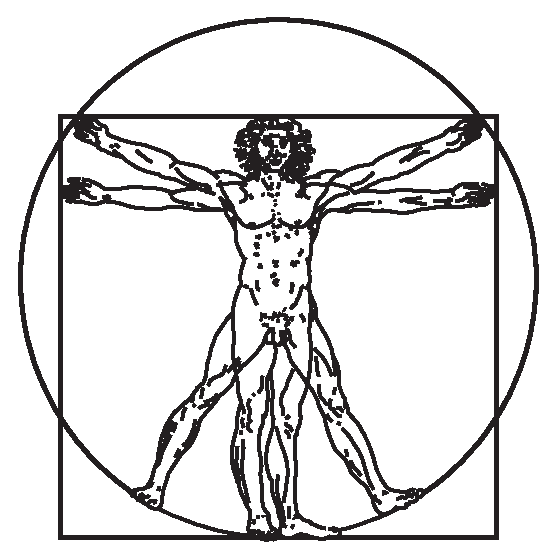
\includegraphics[scale=.5]{emblem}
\label{mmikz-logo}
\caption{Эмблема конференции}
\end{figure}

Ниже (см. табл.~\ref{sampletable}) представлен вариант таблицы с заголовком оформленным с помощью \verb"\caption". 
Если рисунок один, то его заголовок оформляется с помощью \verb"\caption*".

\begin{table}[ht!]
\centering\small
\caption{Пример небольшой таблицы}
\label{sampletable}
\begin{tabular}{|c|c|c|c|c|}
\hline
Номер &~~~~$X$~~~~ &~~~~$Y$~~~~&~~~~$R$~~~~&~~~~Цвет~~~~\\
\hline
\rule{0mm}{12pt}%
1 &	100  &	170 & 30 & красный\\
2 &	100  &	90	& 60 & жёлтый\\
3 &	230  &	250	& 50 & синий\\
4 &	130  &	240 & 60 & зелёный\\
5 & 300  &	130 & 30 & зелёный\\
6 &	200  &	150	& 90 & красный\\
\hline
\end{tabular}
\end{table}

При оформлении формул, рисунков, таблиц и других элементов рукописи рекомендуется использовать книги \cite{latex:book1, latex:book2, latex:book3} или любые другие.


Для составления библиографического списка должен использоваться пакет \href{http://www.mathnet.ru/poffice/amsbibpackage.phtml?wshow=amsbibpackage&option_lang=rus}{\texttt{amsbib}}, руководство к~которому размещено по ссылке \url{http://www.mathnet.ru/poffice/amsbib.pdf}.
Для ссылки на источники необходимо использовать команду \verb"\cite".
На все источники в списке литературы должны быть списки, поэтому не оставим последний элемент нашего библиографического списка без ссылки  \cite{ZhiIza09}.


\section*{Заключение}

Заключение является неотъемлемой частью любой работы. 
Оно должно содержать краткие выводы по результатам исследования, отражающие новизну и~практическую значимость работы, предложения по использованию ее результатов, оценку её эффективности и~качества.

\section*{Благодарности\protect\footnote{Этот раздел статьи может отсутствовать. 
В~него рекомендуется добавлять сведения о финансировании работы и выражать благодарности персонам.}}
%\section*{Благодарности}

Автор настоящего шаблона благодарен Дональду Кнуту за разработку и создание настольной издательской системы \TeX,
Лесли Лэмпорту за разработку макрорасширения \LaTeX\ и Александру Роженко за разработку класса \verb"ncc" и макросов \NCC, которые использовались при разработке макроопределений для этого шаблона.


\begin{thebibliography}{99}
\RBibitem{latex:book1}
\by Котельников~И.~А., Чеботаев~П.~З.
\book Издательская система \LaTeXe
\publaddr Новосибирск
\publ Сибирский хронограф
\yr 1998
\totalpages 496
\morerref
\by Котельников~И.~А., Чеботаев~П.~З.
\book \LaTeX\ по-русски 
\publaddr Новосибирск
\publ Сибирский хронограф
\yr 2004
\totalpages 496


\RBibitem{latex:book2} 
\by Роженко~А.~И. 
\book Искусство верстки в \LaTeX'е
\publaddr Новосибирск
\publ ИВМиМГ СО~РАН
\yr 2005
\totalpages 398

\RBibitem{latex:book3}
\by Балдин~Е.~М. 
\book Компьютерная типография \LaTeX
\publaddr СПб.
\publ БХВ-Петербург
\yr 2008
\totalpages 304

\RBibitem{ZhiIza09}
\by Жижченко~А.~Б., Изаак~А.~Д.
\paper Информационная система Math-Net.Ru. Современное состояние и перспективы развития. Импакт-факторы российских математических журналов
\jour УМН
\yr 2009
\vol 64
\issue 4(388)
\pages 195--204
\transl
\by Zhizhchenko~A.~B., Izaak~A.~D.
\paper The information system Math-Net.Ru. Current state and prospects. The~impact factors of Russian mathematics journals
\jour Russian Math. Surveys
\yr 2009
\vol 64
\issue 4
\pages 775--784

\end{thebibliography}

\section*{Сведения об авторе(ах)\protect\footnote{Сведения об авторе(ах) являются обязательным элементом статьи и приводятся по предлагаемому образцу}}
%\section*{Сведения об авторе(ах)}

\begin{minipage}{\textwidth} 
\small
\noindent \textbf{Саушкин Михаил Николаевич}\footnote{Самарский государственный технический университет, Самара, Россия}, кандидат физико-математических наук, доцент, e-mail: \email{saushkin.mn@samgtu.ru}\par 
%\smallskip
%\noindent \textbf{Фамилия Имя Отчество}\footnote{Аффилированная организация с указанием города и страны}, учёная степень, учёное звание, e-mail: \email{mail@mail.ru}\par
%\smallskip
%\noindent \textbf{Фамилия Имя Отчество}\footnote{Аффилированная организация с указанием города и страны}, студент (аспирант), e-mail: \email{mail@mail.ru} 
\end{minipage}

%\clearpage
%\tableofcontents

\end{document}